\chapter{Neo4j}

\begin{wrapfigure}{l}{0.3\textwidth}
  \vspace{-75pt}
  \begin{center}
    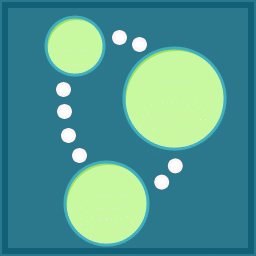
\includegraphics[width=0.28\textwidth]{neo4j.png}
  \end{center}
  \vspace{-30pt}
\end{wrapfigure}
Neo4j is an open-source graph database, implemented in Java. The developers describe Neo4j as <<embedded, disk-based, fully transactional Java persistence engine that stores data structured in graphs rather than in tables>>. The community edition of the database is licensed under the free GNU General Public License (GPL) v3. The additional modules, such as online backup and high availability, are licensed under the free Affero General Public License (AGPL) v3. The database, with the additional modules, is also available under a commercial license, in a dual license model.

\section{Short specification}

\begin{itemize}
  \item \textbf{Written in:} Java
  \item \textbf{Main point:} Graph database
  \item \textbf{License:} Dual-licensed: GPLv3 and AGPLv3 / commercial
  \item \textbf{Protocol:} HTTP/REST (or embedding in Java)
  \item \textbf{Web site:} \href{http://neo4j.org/}{neo4j.org}
\end{itemize}

\section{Main features}

\section{Strengths}

Neo4j is one of the finest examples of open source graph databases. Graph databases are perfect for unstructured data, in many ways even more so than document datastores. Not only is Neo4j typeless and schemaless, but it puts no constraints on how data is related. It is, in the best sense, a free-for-all. Currently, Neo4j can support 34.4 billion nodes and 34.4 billion relationships, which is more than enough for most uses (Neo4j could hold more than 42 nodes for each of Facebook’s 800 million users in a single graph).

The Neo4j distributions provide several tools for fast lookups with Lucene and easy-to-use (if sometimes cryptic) language extensions like Gremlin and the REST interface. Beyond ease of use, Neo4j is fast. Unlike join operations in relational databases or map-reduce operations in other databases, graph traversals are constant time. Like data is only a node step away, rather than joining values in bulk and filtering the desired results—as most of the databases we’ve seen operate. It doesn’t matter how large the graph becomes; moving from node A to node B is always one step if they share a relationship. Finally, the Enterprise edition provides for highly available and high read- traffic sites by way of Neo4j HA.\cite{seven_databases}

\section{Weaknesses}

Neo4j does have a few shortcomings. Edges in Neo4j cannot direct a vertex back on itself. We also found its choice of nomenclature (node rather than vertex, and relationship rather than edge) to add complexity when communicating. Although HA is excellent at replication, it can only replicate a full graph to other servers. It cannot currently shard subgraphs, which still places a limit on graph size (though, to be fair, that limit measures in the tens of billions). Finally, if you are looking for a business-friendly open source license (like MIT), Neo4j may not be for you. Where the Community edition (everything we used in the first two days) is GPL, if you want to run a production environment using the Enterprise tools (which includes HA and backups), you’ll probably need to purchase a license.\cite{seven_databases}

\section{Tips}

\section{Use cases}

\begin{itemize}
  \item Session Storage
  \item Cache Storage
  \item Job Queue
  \item Real time analysis
  \item Pub/Sub
\end{itemize}